\documentclass[frenchb,francais]{beamer}
\usepackage[francais]{babel}
\usepackage[T1]{fontenc}
\usepackage[utf8x]{inputenc}
\usepackage{ulem}
\DeclareSymbolFont{extraup}{U}{zavm}{m}{n}
\DeclareMathSymbol{\varheart}{\mathalpha}{extraup}{86}
\usepackage{dirtree}
\usepackage{hyperref}

\usepackage{listings}
\usepackage{color}

\definecolor{dkgreen}{rgb}{0,0.6,0}
\definecolor{gray}{rgb}{0.5,0.5,0.5}
\definecolor{mauve}{rgb}{0.58,0,0.82}

\lstset{frame=tb,
  language=Python,
  aboveskip=3mm,
  belowskip=3mm,
  showstringspaces=false,
  columns=flexible,
  basicstyle={\footnotesize\ttfamily},
  numbers=none,
  numberstyle=\tiny\color{gray},
  keywordstyle=\color{blue},
  commentstyle=\color{dkgreen},
  stringstyle=\color{mauve},
  breaklines=true,
  breakatwhitespace=true,
  tabsize=4,
  captionpos=n
}

\usetheme{PaloAlto}
\usepackage{graphicx}

\usecolortheme{seagull}

\logo{
\includegraphics[height=10mm]{img/Python-logo-notext.png}}


\title[Pelican]{Pelican : le futur du web vintage}
\author {Damien Nicolas}

\AtBeginSection{
  \begin{frame}
  \frametitle{Plan}
  \tableofcontents[currentsection]
  \end{frame}
}

%\useoutertheme[right,width=2cm]{sidebar}

\begin{document}

\frame{\titlepage}

\begin{frame}
\frametitle{Plan}
\tableofcontents
\end{frame}

\section{Quoi ?}

\begin{frame}
    \frametitle{Quoi ?}
    \begin{center}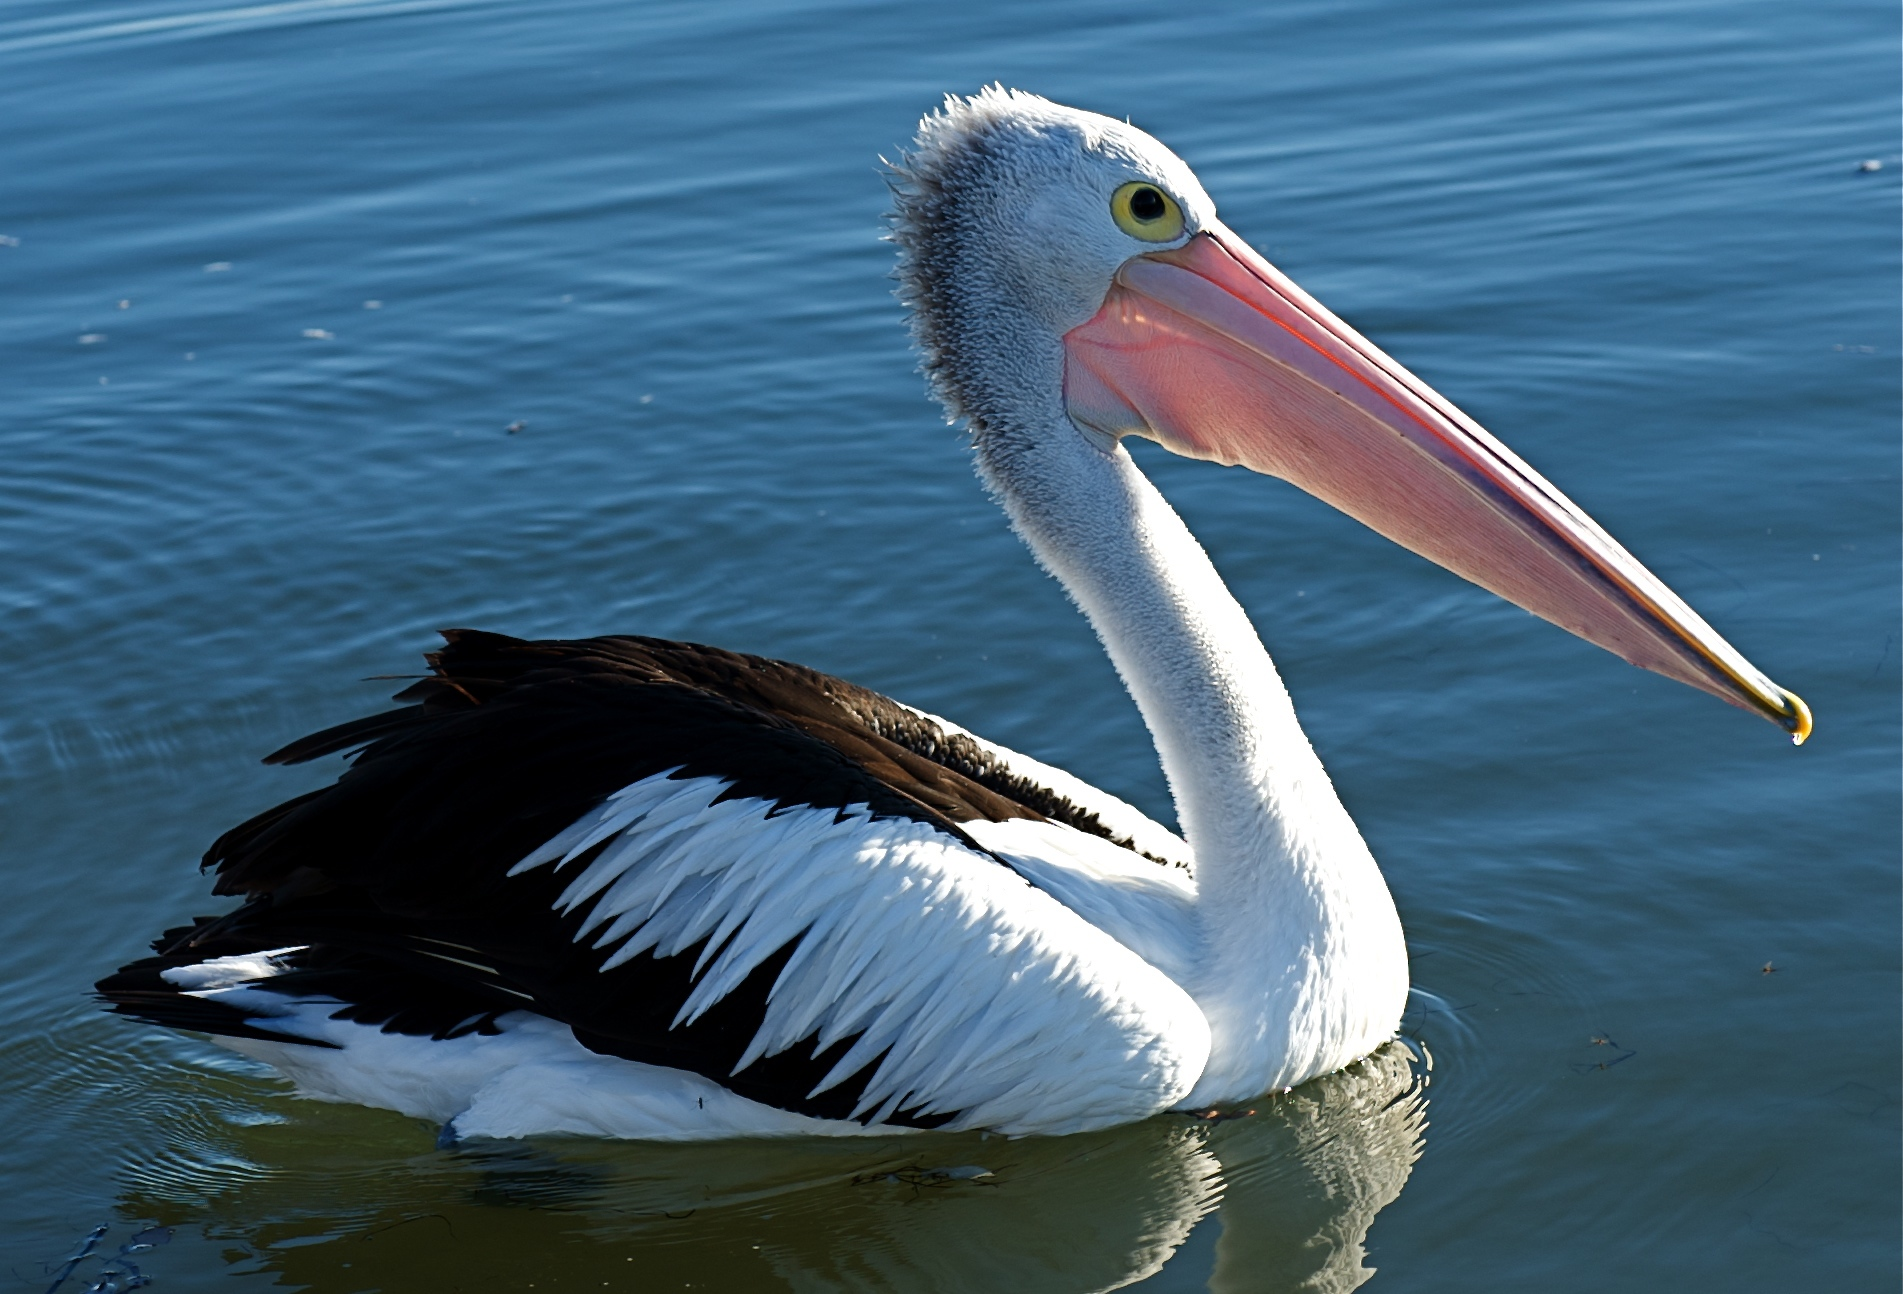
\includegraphics[scale=.08]{img/pelican.jpg}\end{center}
    \begin{itemize}
        \item Générateur de sites statiques
        \item Écrit en pure-Python, tourne sous Cpython 2.7, 3.3 et 3.4
        \item Initié par Alexis Métaireau
        \item Débuté en août 2010, activement maintenu, plus de 200 contributeurs
    \end{itemize}
\end{frame}

\begin{frame}
    \frametitle{Principe}
    \begin{center}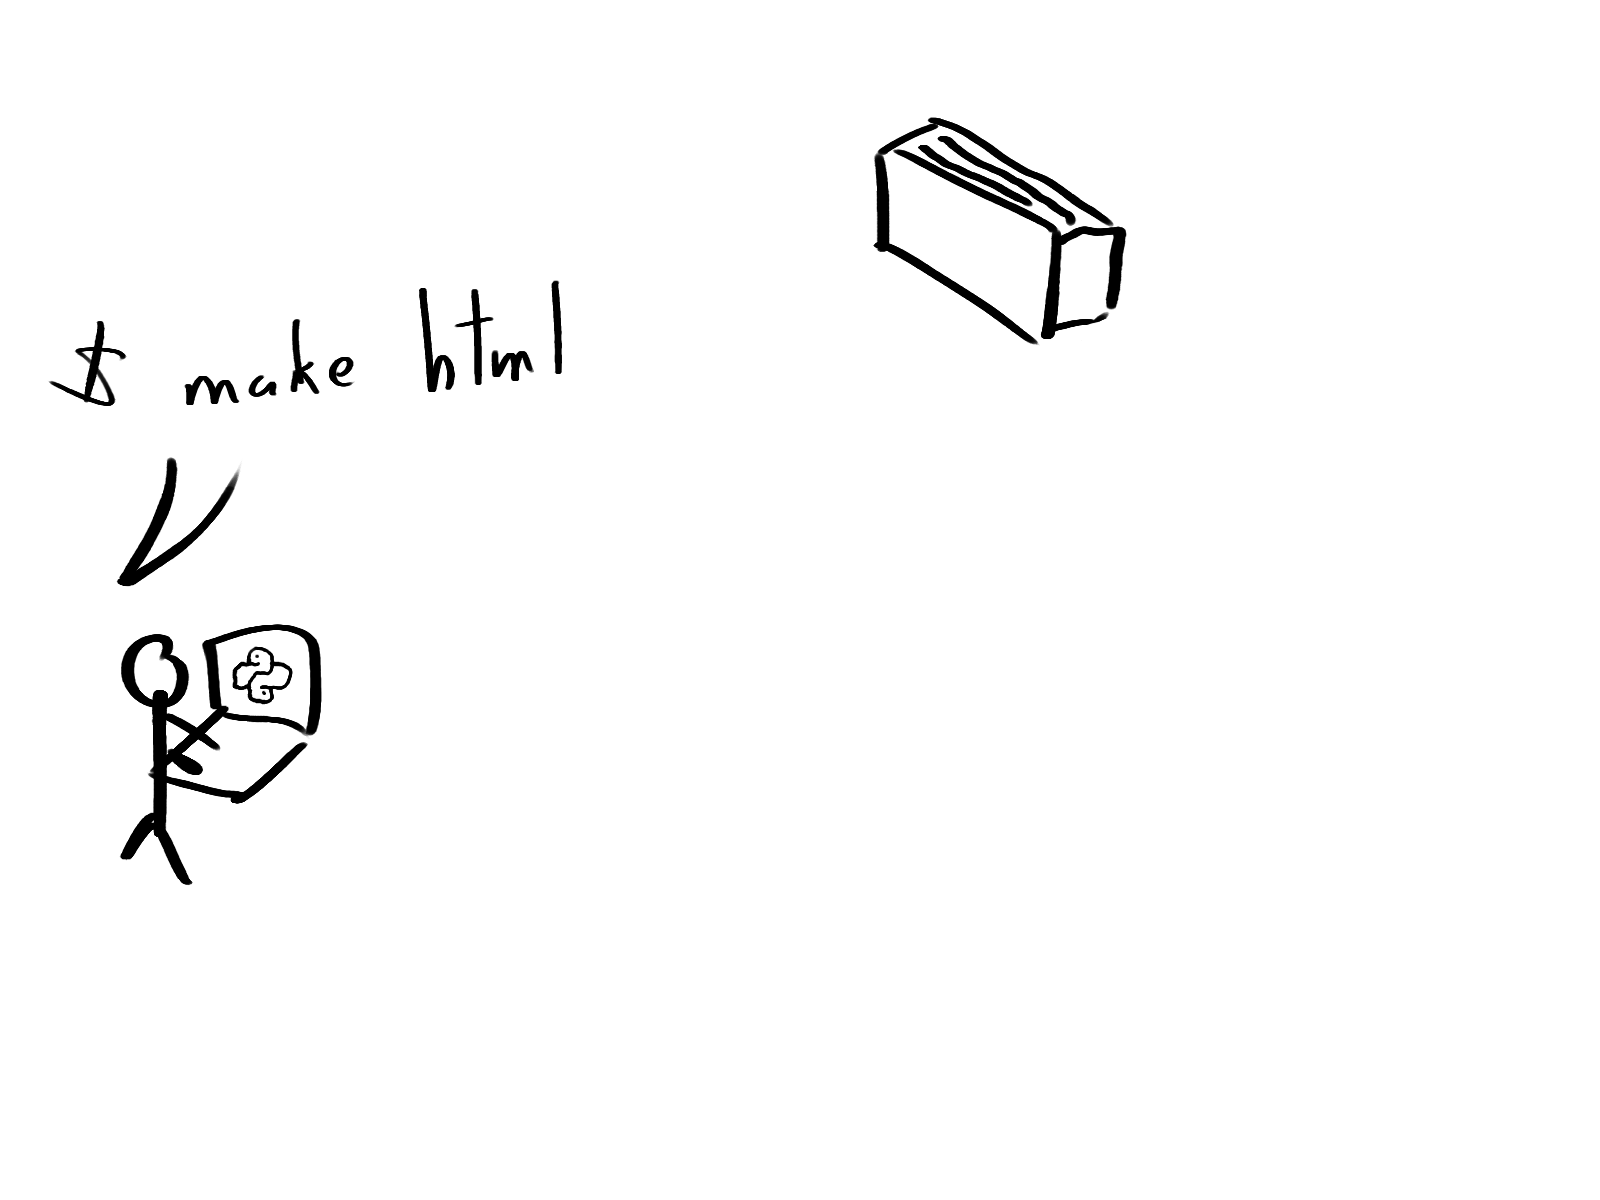
\includegraphics[scale=.20]{img/static-generation_1.png}\end{center}
\end{frame}

\begin{frame}
    \frametitle{Principe}
    \begin{center}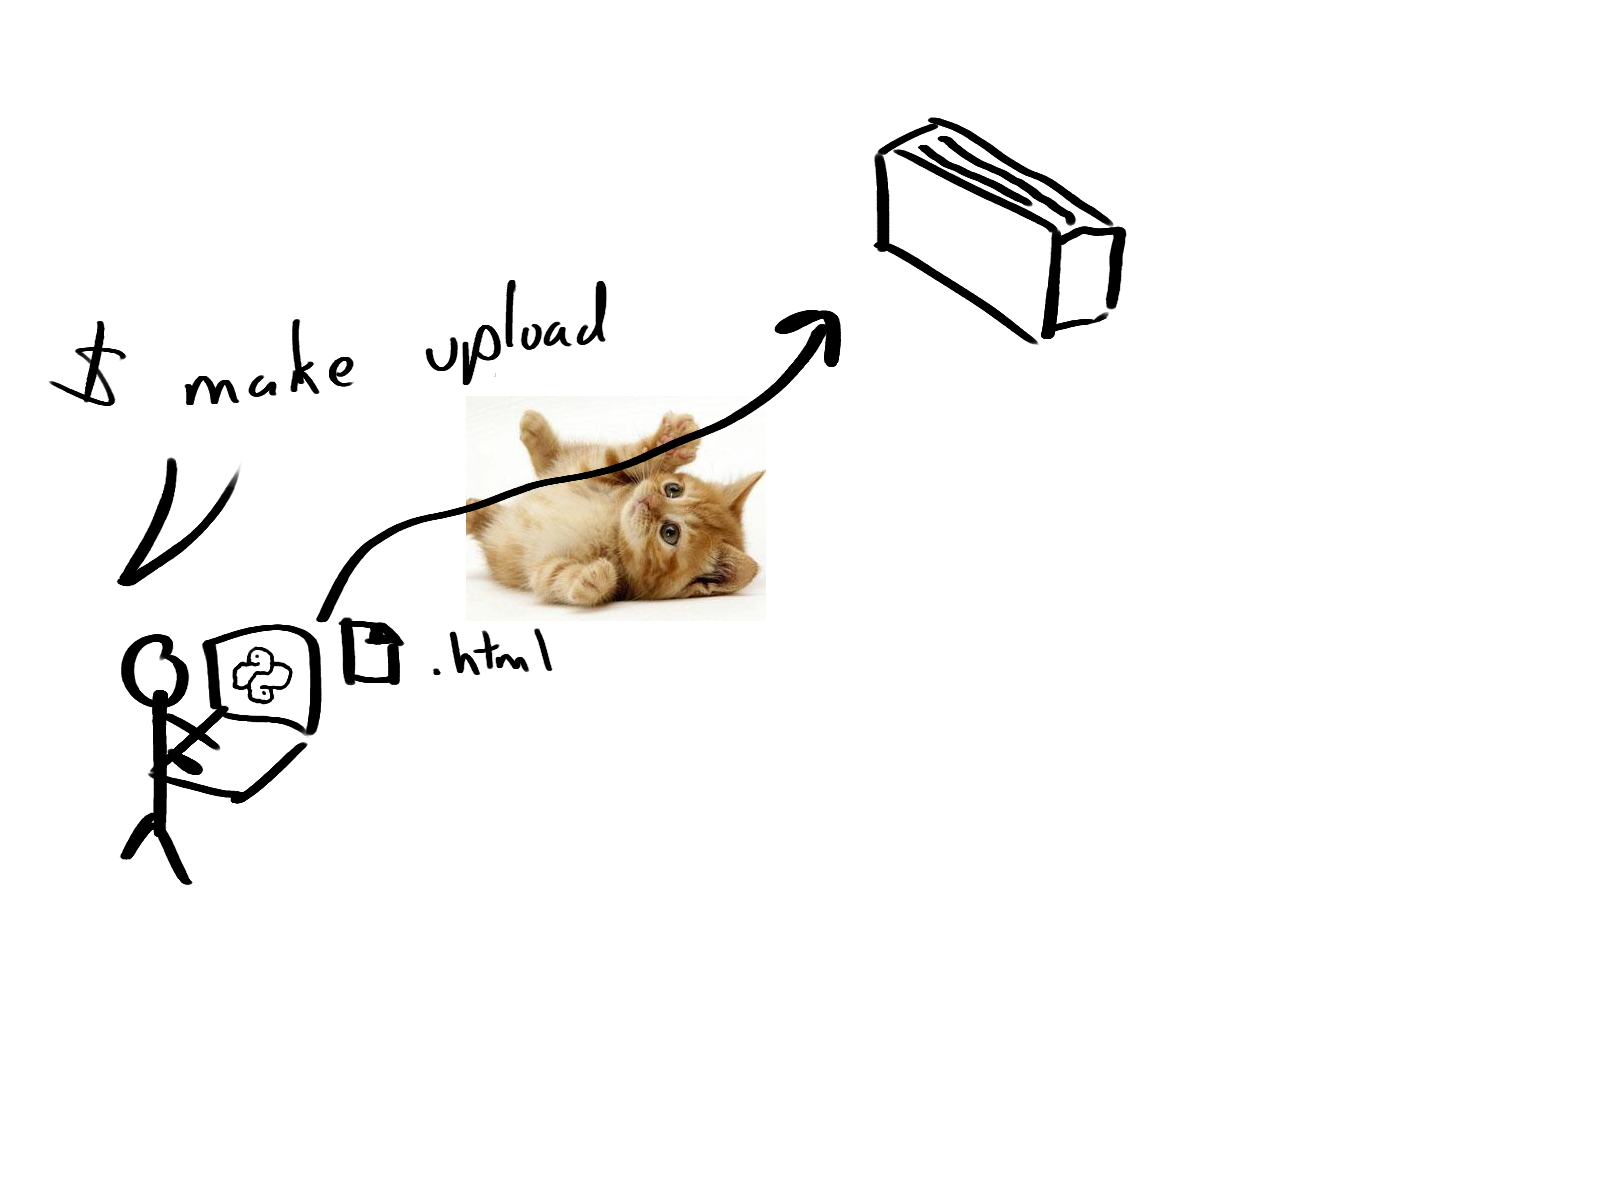
\includegraphics[scale=.20]{img/static-generation_2.png}\end{center}
\end{frame}

\begin{frame}
    \frametitle{Principe}
    \begin{center}
\includegraphics[scale=.20]{img/static-generation_3.png}\end{center}
\end{frame}

\section{Pourquoi ?}

\begin{frame}
    \frametitle{Performance}
    \begin{center}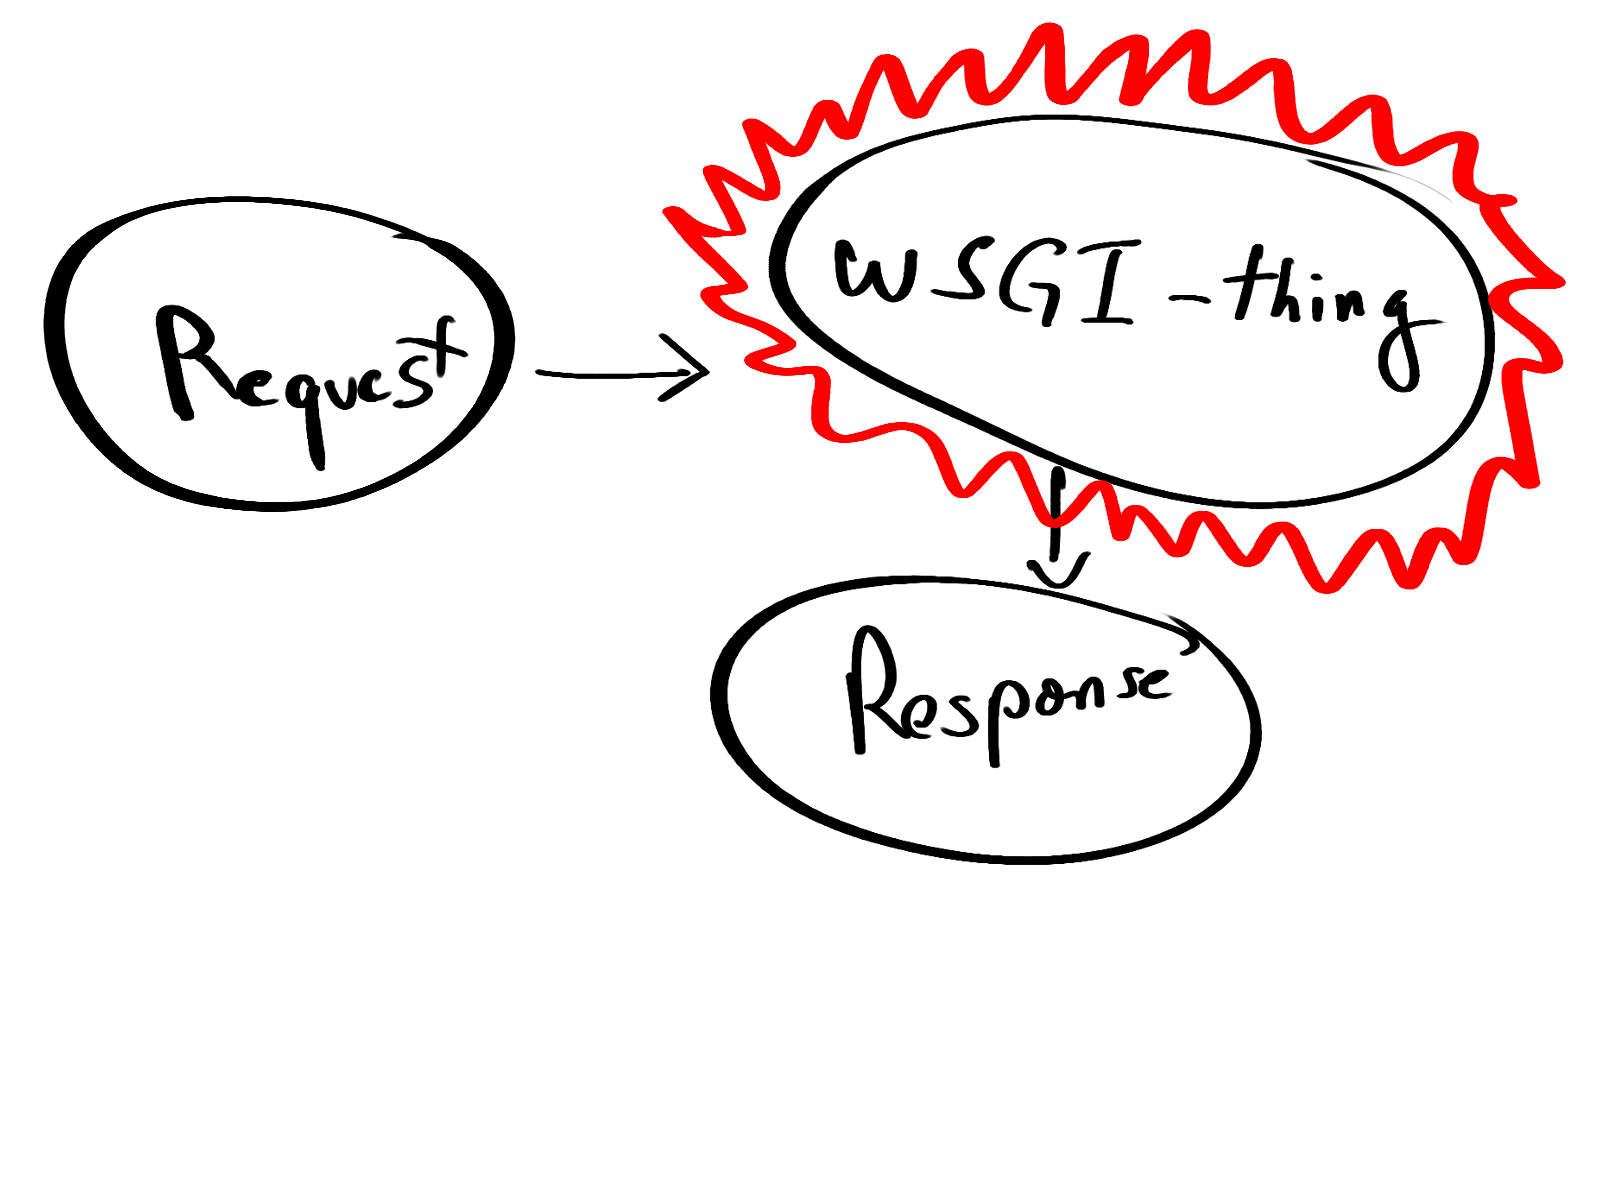
\includegraphics[scale=.17]{img/wsgi-flow.png}\end{center}
\end{frame}

\begin{frame}
    \frametitle{Performance}
    \begin{center}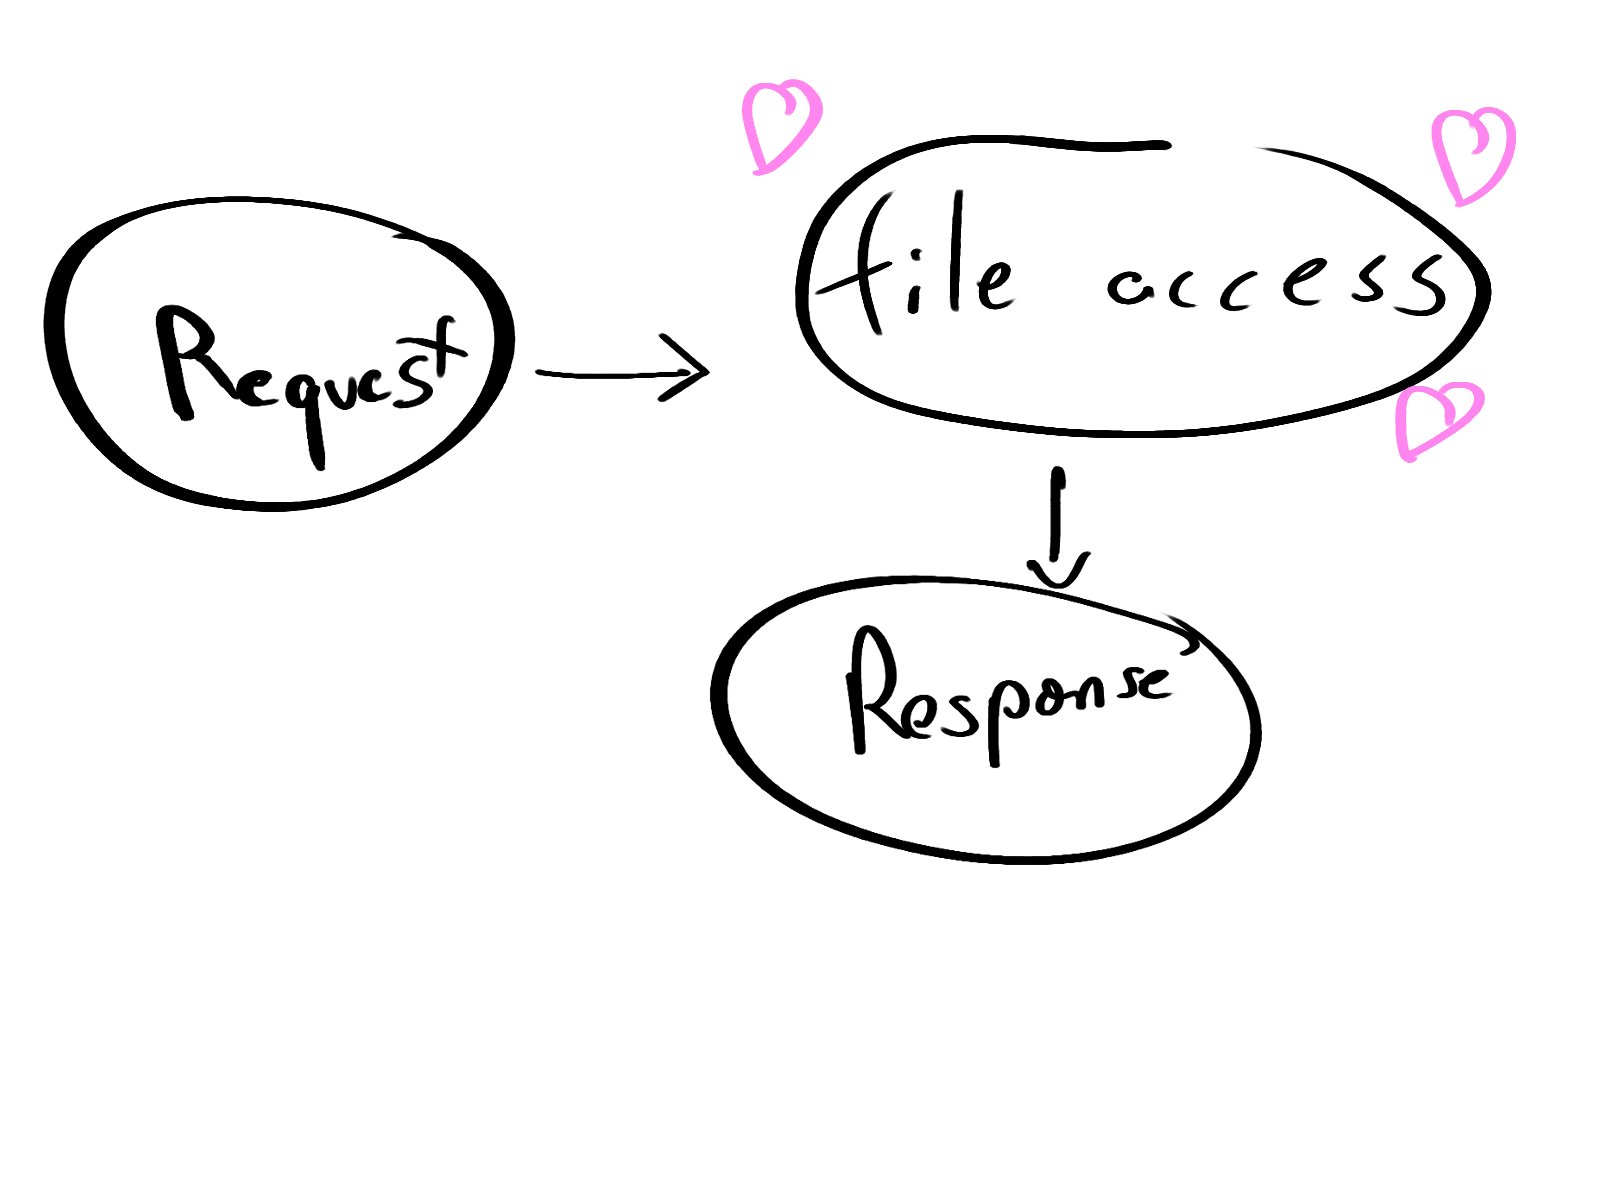
\includegraphics[scale=.17]{img/pelican-flow.png}\end{center}
\end{frame}

\begin{frame}
    \frametitle{Performance}
    \begin{center}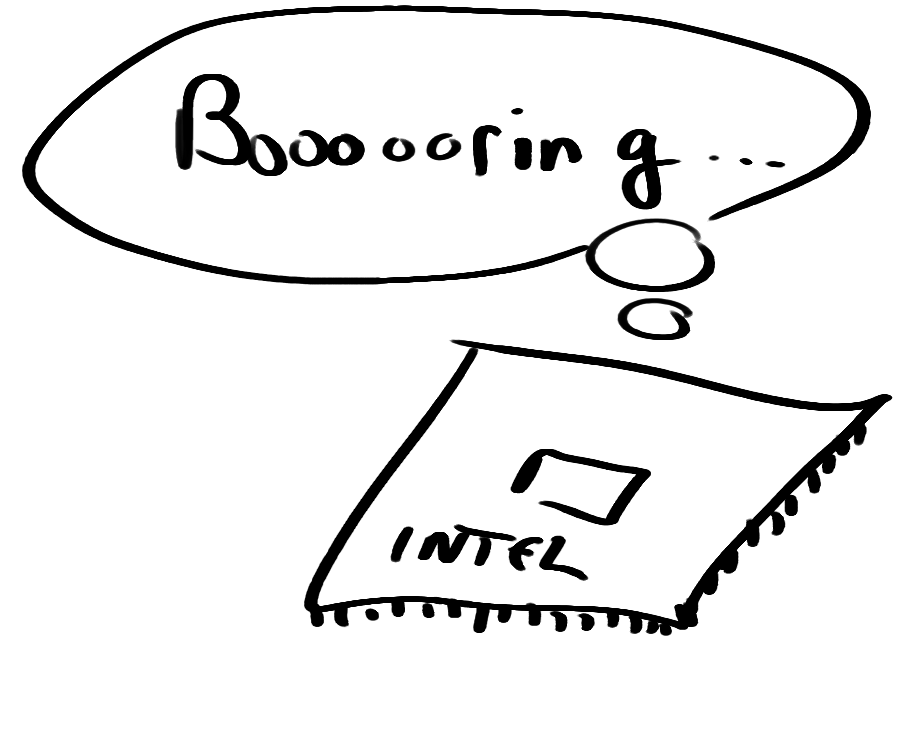
\includegraphics[scale=.15]{img/boring.png}\end{center}
    Le temps de calcul côté serveur est réduit à néant. Difficile de faire moins
    coûteux que des fichiers statiques.
\end{frame}

\begin{frame}
    \frametitle{Sécurité}
    \begin{center}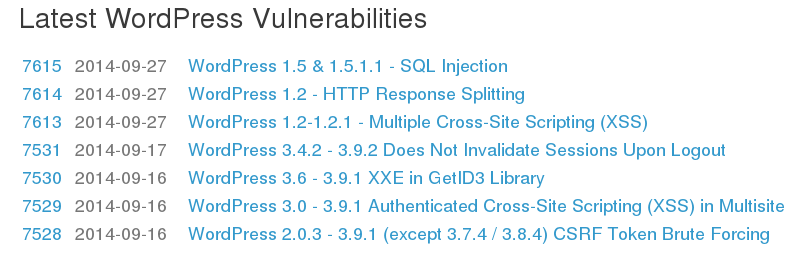
\includegraphics[scale=.30]{img/wordpress-security.png}\end{center}
    Zéro faille applicative dans du HTML
\end{frame}

\begin{frame}
    \frametitle{Praticité}
    \begin{itemize}
        \item J’aime écrire mes billets sous Vim
        \item On m’envoie des patches correctifs par mails chiffrés $\varheart$
        \item Ça s’intègre proprement dans un VCS
    \end{itemize}
\end{frame}

\begin{frame}
    \frametitle{Les inconvénients}
    \begin{itemize}
        \item Il n’y a pas de commentaires
        \item Recherche impossible
        \item Barrière technique plus importante qu’avec un Wordpress
    \end{itemize}
\end{frame}

\begin{frame}
    \frametitle{Pas de commentaires}
    \begin{center}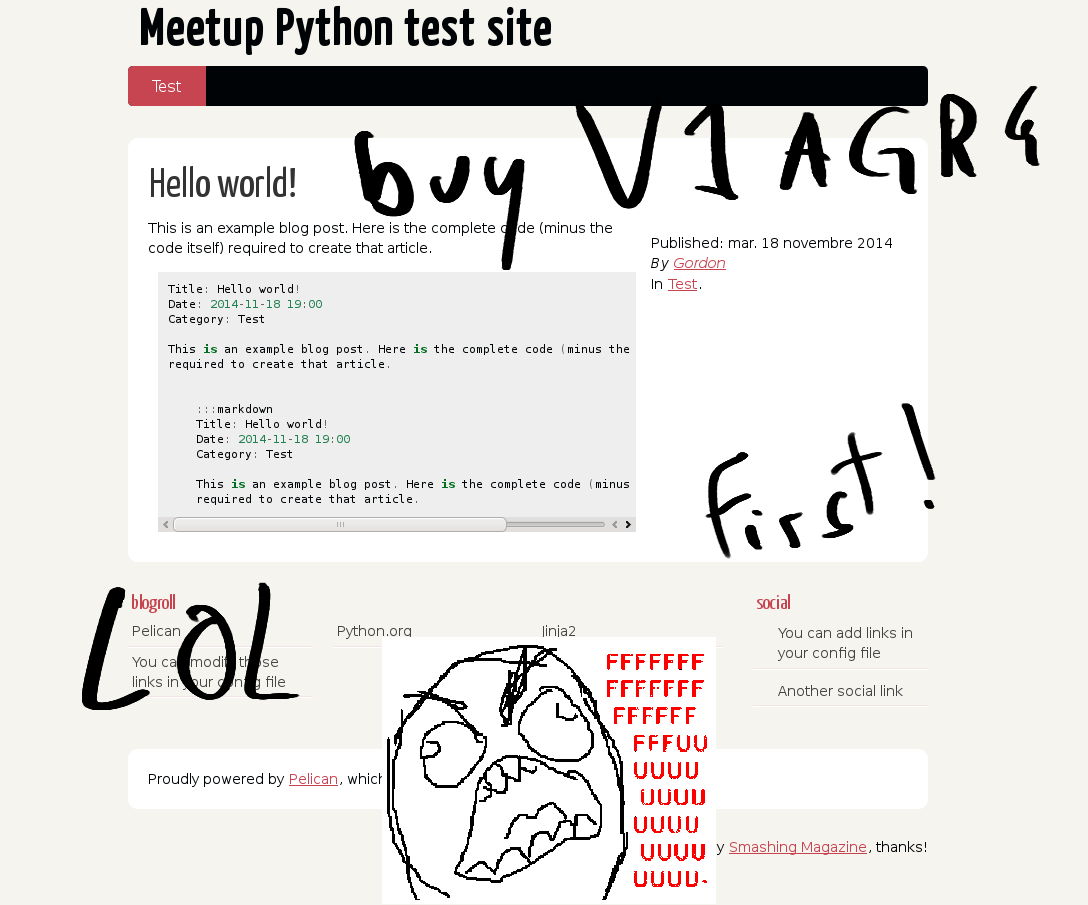
\includegraphics[scale=.17]{img/comments_2.png}\end{center}
\end{frame}

\section{Comment ?}

\begin{frame}
    \frametitle{Prérequis}
    \begin{itemize}
        \item Python (si vous avez encore une 2.6, upgradez, par pitié)
        \item (optionnel) virtualenv
        \item (optionnel) git ou un autre VCS
    \end{itemize}
\end{frame}

\begin{frame}[containsverbatim]
    \frametitle{Installation}
    \lstset{language=bash}
    \begin{lstlisting}
$ virtualenv pelican
$ source pelican/bin/activate
$ pip install pelican Markdown
$ pelican-quickstart
    \end{lstlisting}
\end{frame}

\begin{frame}
    \frametitle{Quickstart}
    \begin{center}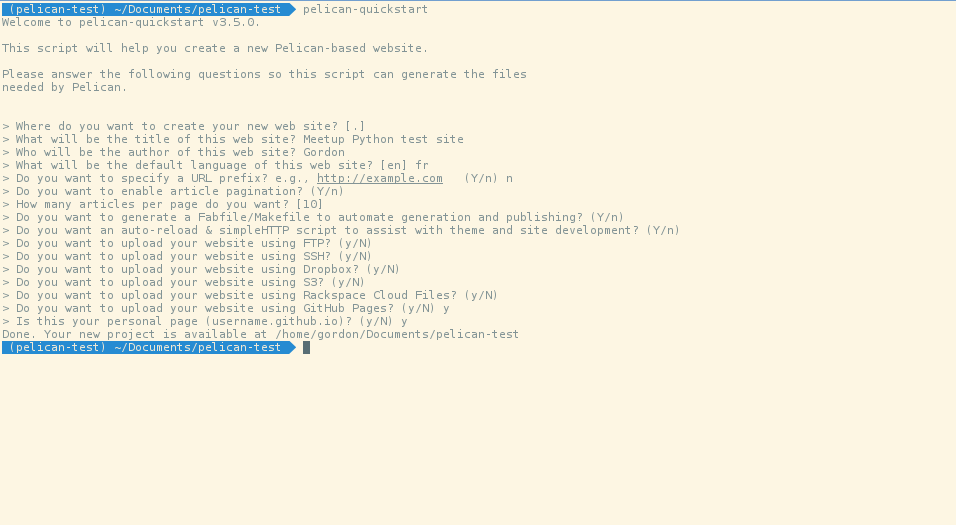
\includegraphics[scale=.30]{img/quickstart.png}\end{center}
\end{frame}

\begin{frame}[containsverbatim]
    \frametitle{Arborescence}
\dirtree{%
.1 pelican-test.
.2 content.
.3 (pages).
.2 output.
.2 develop\_server.sh.
.2 fabfile.py.
.2 Makefile.
.2 pelicanconf.py.
.2 publishconf.py.
}
\end{frame}

\begin{frame}[containsverbatim]
    \frametitle{Premier article}
    \begin{lstlisting}
Title: Hello world!
Date: 2014-11-18 19:00
Category: Test

This is an example blog post. Here is the complete code (minus the code itself)
required to create that article.

    :::markdown
    Title: Hello world!
    Date: 2014-11-18 19:00
    Category: Test

    This is an example blog post. Here is the complete code (minus the code itself)
    required to create that article.
    \end{lstlisting}
\end{frame}

\begin{frame}[containsverbatim]
    \frametitle{Compilation}
    \lstset{language=bash}
    \begin{lstlisting}
$ make html
pelican /home/gordon/Documents/pelican-test/content -o /home/gordon/Documents/pelican-test/output -s /home/gordon/Documents/pelican-test/pelicanconf.py 
Done: Processed 1 article(s), 0 draft(s) and 0 page(s) in 0.16 seconds.
$ make serve # puis on ouvre un navigateur sur http://127.0.0.1:8000
cd /home/gordon/Documents/pelican-test/output && python3 -m pelican.server
    \end{lstlisting}
\end{frame}

\begin{frame}
    \frametitle{Et voilà !}
    \begin{center}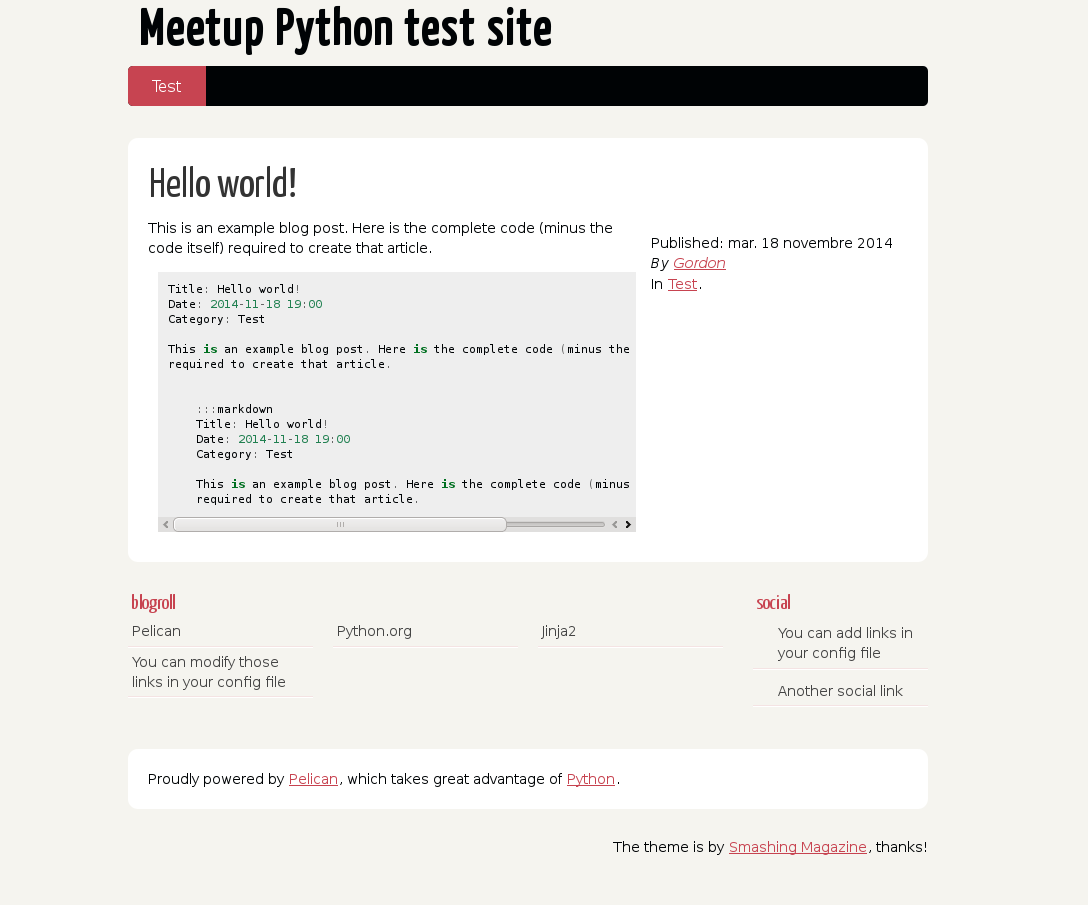
\includegraphics[scale=.20]{img/comments.png}\end{center}
\end{frame}

\begin{frame}
    \frametitle{Configuration}
    \begin{center}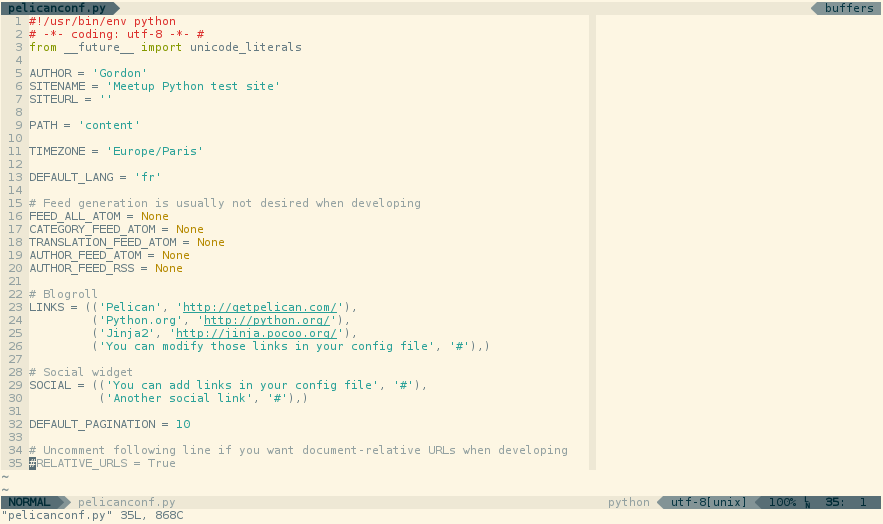
\includegraphics[scale=.34]{img/pelicanconf.png}\end{center}
\end{frame}

\section{Quel goût ça a ?}

\begin{frame}
    \frametitle{Templating}
    \begin{center}
\includegraphics[scale=.15]{img/jinja.png}\end{center}
\end{frame}

\begin{frame}
    \frametitle{Templating}
    \begin{center}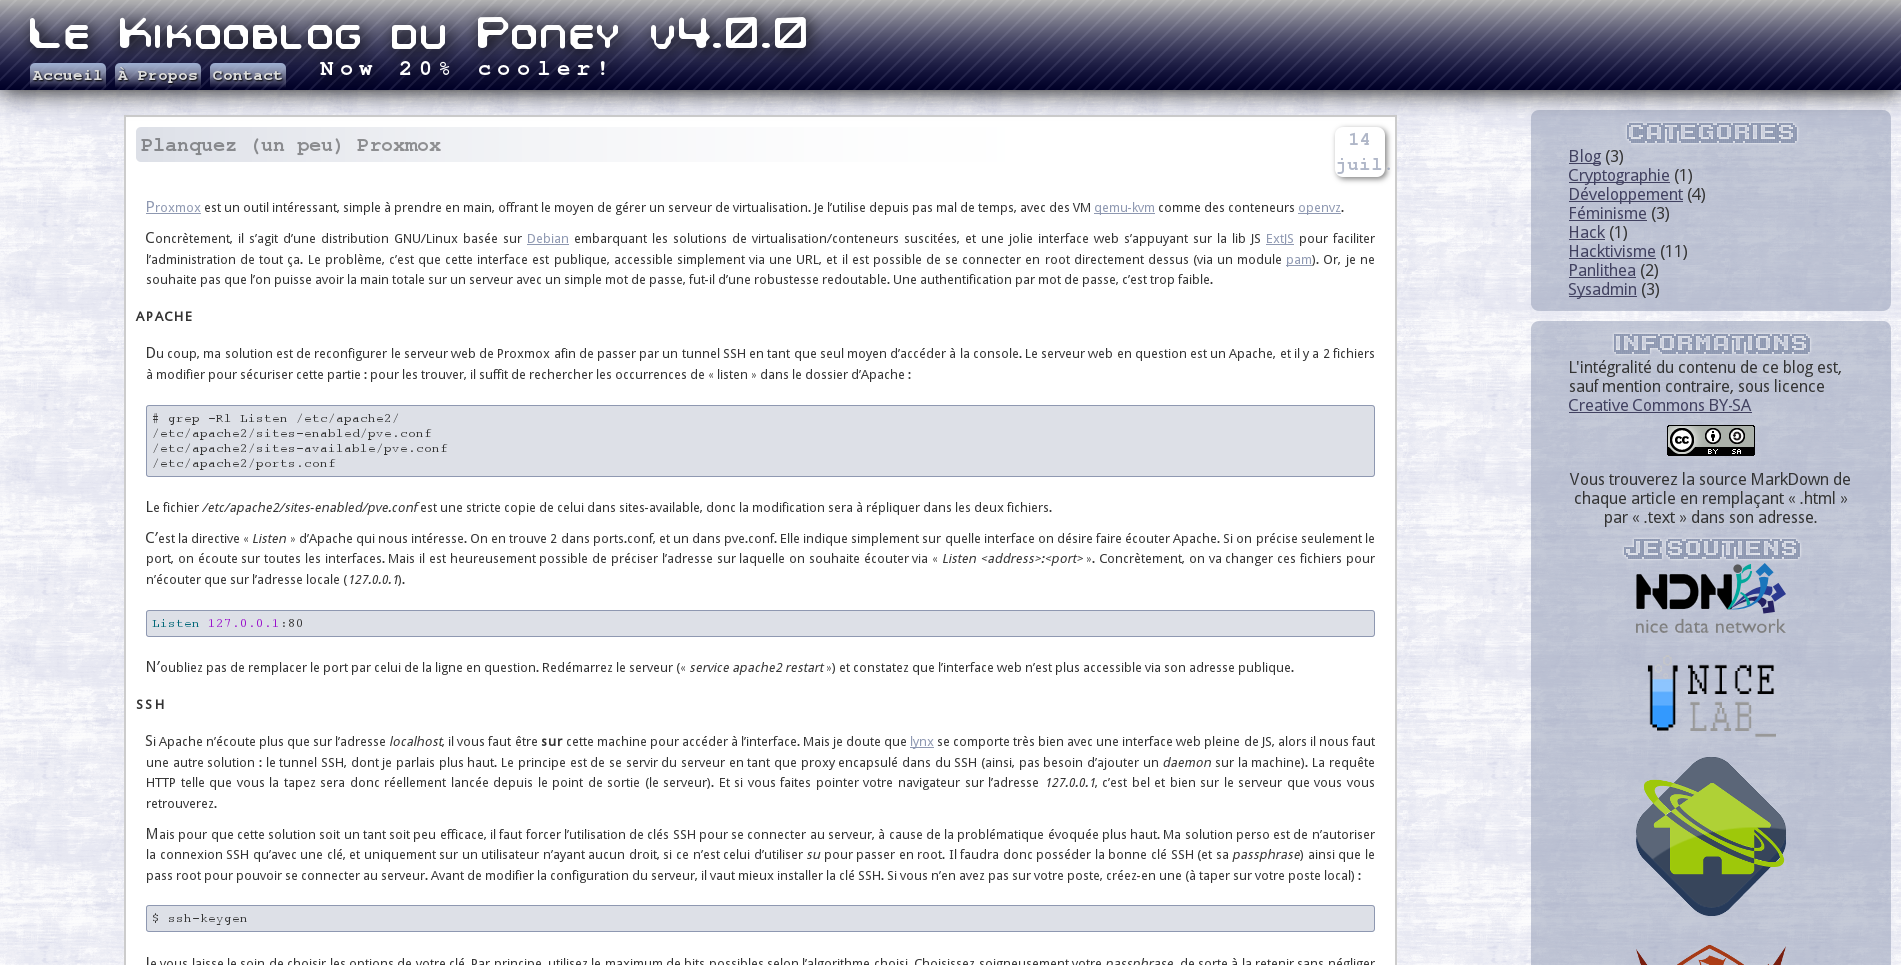
\includegraphics[scale=.15]{img/gordon_re.png}\end{center}
\end{frame}

\begin{frame}
    \frametitle{Templating}
    \begin{center}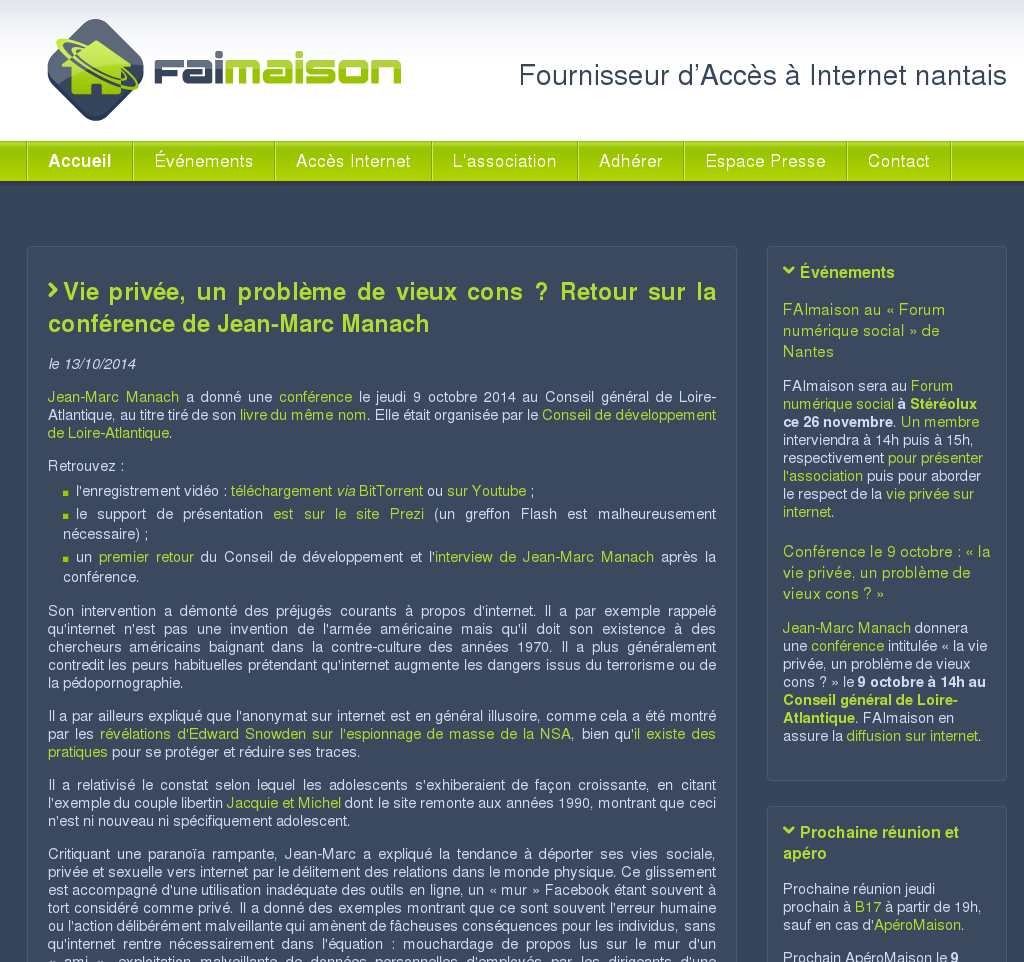
\includegraphics[scale=.20]{img/faimaison_net.png}\end{center}
\end{frame}

\begin{frame}
    \frametitle{Templating}
    \begin{center}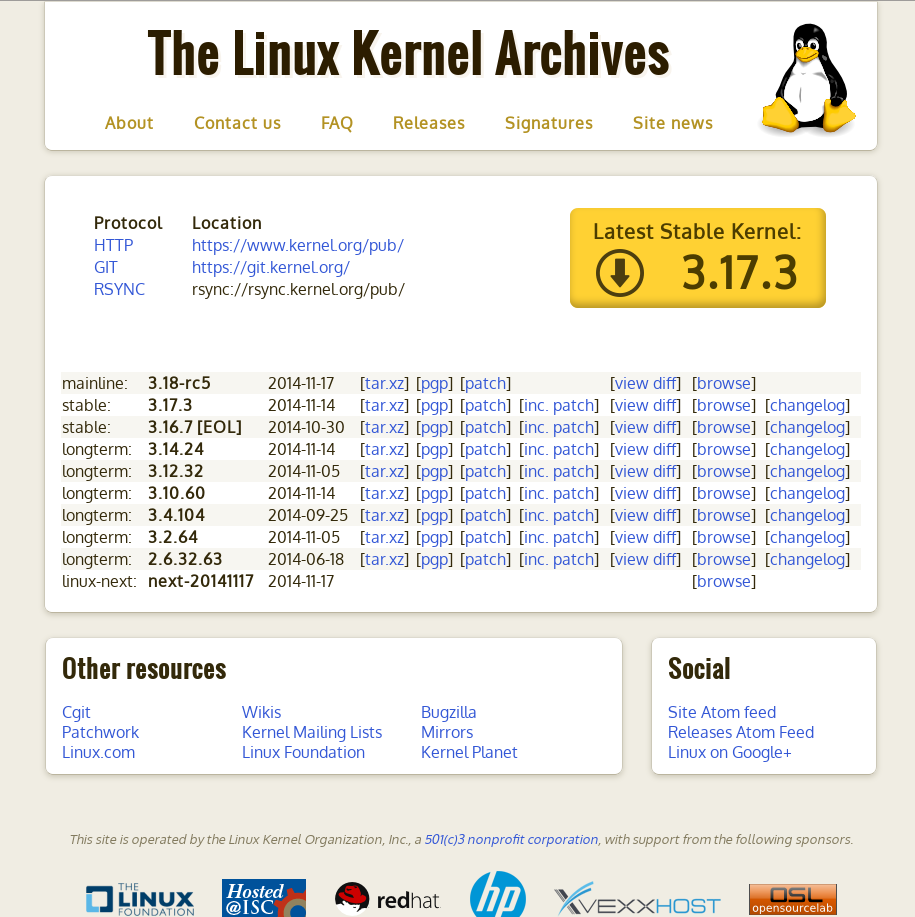
\includegraphics[scale=.20]{img/kernel_org.png}\end{center}
\end{frame}

\begin{frame}
    \frametitle{Commentaires externes}
    \begin{center}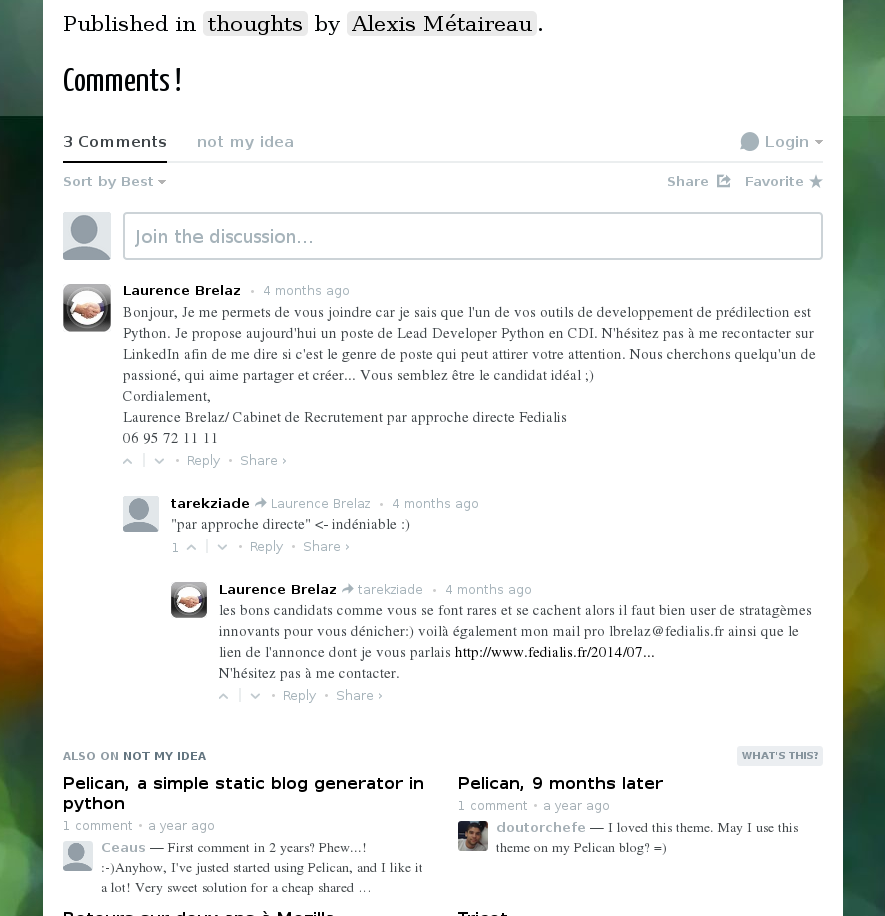
\includegraphics[scale=.20]{img/disqus.png}\end{center}
\end{frame}

\begin{frame}
    \frametitle{Commentaires externes, bis}
    Vous non plus, vous n’aimez pas Disqus et les machins fermés ?
    \begin{itemize}
        \item Isso [\url{http://posativ.org/isso}]
        \item Discourse [\url{https://discourse.org}]
        \item Commentaires statiques
    \end{itemize}
\end{frame}

\begin{frame}
    \frametitle{Plugins}
    \begin{center}
\includegraphics[scale=.12]{img/plugins.png}\end{center}
\end{frame}

\begin{frame}
    \frametitle{Plugins}
    \begin{center}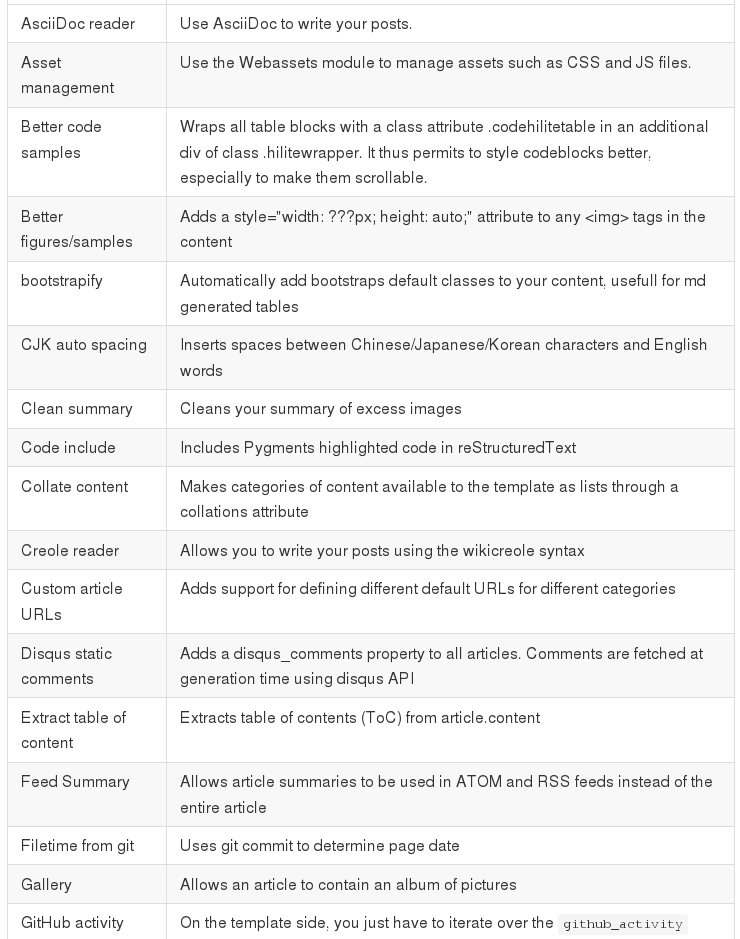
\includegraphics[scale=.20]{img/plugin_list.png}\end{center}
\end{frame}

\begin{frame}
    \frametitle{Recherche}
    \begin{center}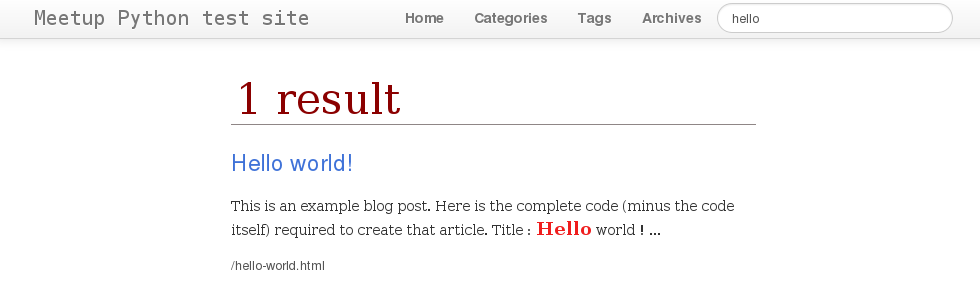
\includegraphics[scale=.20]{img/search.png}\end{center}
    Plugin Tipue-search + theme Elegant
\end{frame}

\section{Et Afpy-Nantes ?}

\begin{frame}
    \frametitle{Sur Github}
    \begin{center}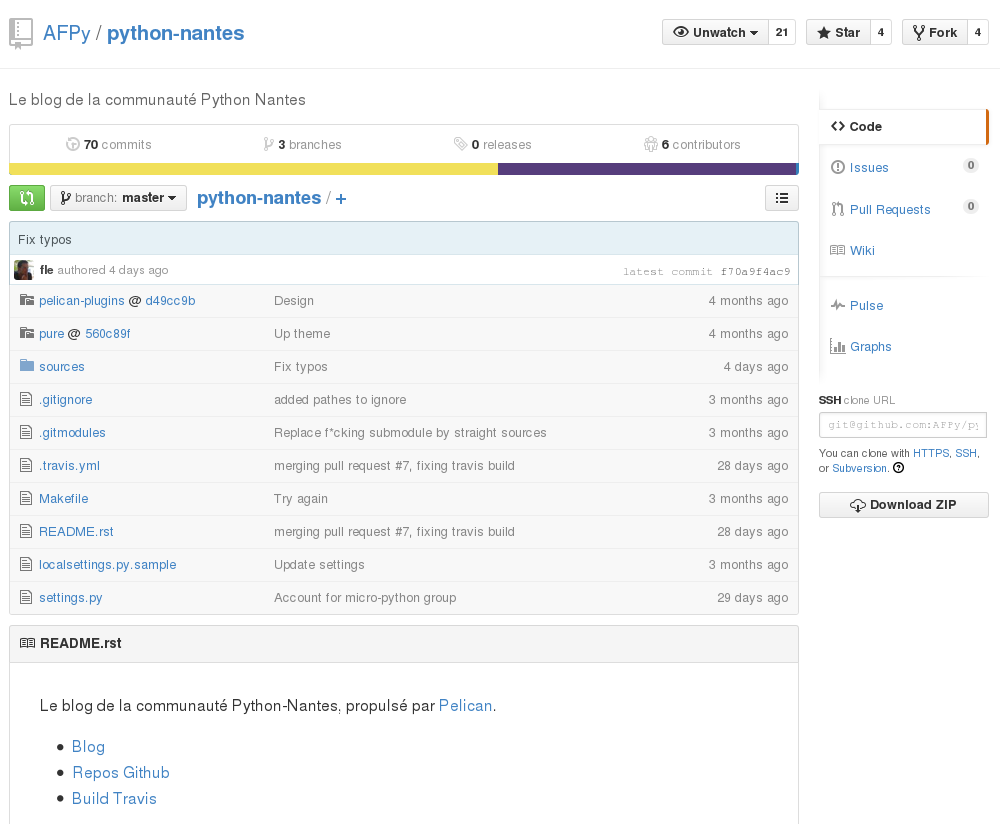
\includegraphics[scale=.20]{img/github.png}\end{center}
\end{frame}

\begin{frame}
    \frametitle{Contribuer}
    \begin{enumerate}
        \item Forker le dépôt
        \item Adapter le localsettings.py
        \item Écrire
        \item Compilation et relecture locale
        \item Commit puis push
        \item Travis fait le reste !
    \end{enumerate}
\end{frame}

\begin{frame}
\frametitle{Questions ?}
\begin{center}
\includegraphics[scale=.40]{img/questions.png}\end{center}
\end{frame}

\end{document}

